\documentclass[../main/thesis]{subfiles}
\graphicspath{{/home/arefk/uio/MScThesis_AreKvanum2022_SeaIceML/thesis/model_development/figures/}}
\begin{document}

\section{Model development}
\label{sec:developing a unet}
This section will cover the implementation of the U-Net architecture, as well as related processes such as data preparation and writing a custom dataloader. Furthermore, this section will present intermediate results obtained during development to highlight technical decisions made as well as their consequence for model performance. Decisions made will be highlighted from both a MachineLearning paradigm point of view, although when relevant they will also be explored in a context of the underlying physics.

\subsection{Data preprocessing}
The deep learning system can be disassembled into two parts, a dataloader followed by the deep learning model itself. The dataloader structures already preprocessed data which it feeds the deep learning model during training. However, the data which is included in a sample is delivered on different spatial grids and resolutions, as well as being exposed to computations which structure the spatiotemporal information. As such, preparatory work which would limit training speed or require more memory than strictly necessary are done in advance.

An overview of the data pipeline and workflow is described in figure (\ref{fig:data_pipeline}). The raw data is sampled from the sea ice charts \citep{Dinessen2020}, OSI SAF SSMIS \citep{Tonboe2017} and AROME Arctic \citep{Mueller2017}. As can be seen from figure (\ref{fig:data_pipeline}), a sample is constructed from a recent sea ice chart, the computed sea ice concentration trend over a set amount of previous days from OSI SAF, recent AROME Arctic 2 meter temperature and wind forecasts as well as a land sea mask, which is the same land sea mask used in AROME Arctic.

\begin{figure}
    \centering
    \includestandalone[width=.865\textwidth]{/home/arefk/uio/MScThesis_AreKvanum2022_SeaIceML/thesis/model_development/figures/pipeline}
    \caption{\label{fig:data_pipeline} Workflow figure providing a overview of the data pipeline. Data is sampled from four sources (Recent Sea Ice Chart, OSI SAF, AROME Arctic and a Land Sea Mask), preprocessed and merged into a single sample. The sample is fed into the network  together with an associated ground truth target sea ice chart. The predicted sea ice chart is compared against the ground truth sea ice chart, and their binary cross entropy error is propagated backwards throughout the network, which constitutes a step in the training loop.}
\end{figure}

\subsubsection{Regridding data}
\label{sec:regrid}
All input data loaded into the U-Net is on the AROME Arctic projection with a 1km spatial resolution and covering the same domain as required by the input layer of the U-Net architecture \citep{Ronneberger2015}. For geographic data, this requirement implies that all data used for training, validation or testing of the deep learning system has to be on a common projection as well as sharing the same grid points. As such, following the region of interest outlined in section (\ref{sec:roi}), the sea ice charts described in section (\ref{sec:data_seaicecharts}) are used as the reference for the domain as they are already supplied on the desired projection and spatial resolution. Other products which are not on the AROME Arctic grid \citep{Mueller2017} or on a 1km spatial resolution \citep{Dinessen2020} have to be reprojected and resampled to match the target grid.

For this work, the process of re-projecting and interpolation is performed on a per-product basis as part of the preprocessing routine. Re-projection of the coordinate data is performed with the Python library \textbf{Pyproj} \citep{Snow2022}, while interpolation onto the new coordinate system is done using nearest neighbor interpolation. In cases where the data is already present on the desired projection, but on a different resolution than the target, only nearest neighbor resampling is performed.

\subsubsection{Sea Ice Charts}
\label{sec:data_seaicecharts}
The sea ice charts used for this thesis has been made available by Nick Hughes of the Norwegian Ice Service. Hughes' work has involved readying the sea ice charts by gridding the dataset from a GIS production environment \citep{Dinessen2020} where concentration contours are drawn onto a 1km spatial resolution grid with the AROME Arctic projection and domain \citep{Mueller2017}. Nearest neighbor interpolation is used when projecting the polygons onto the AROME Arctic grid (Nick Hughes, 2022, pers. commun.). Moreover, the drawn vector polygons run under land, such that all the sea ice charts are fully consistent fields with no missing values. However, there is no systematicity to how the land pixels have been treated, and it has been advised by Hughes to mask out the land by the use of the landmask from AROME Arctic (Nick Hughes, 2022, pers. commun.).

Since the U-Net architecture imposes the restriction that all input data need valid data for entries \citep{Ronneberger2015}, two different methods filling the masked land pixels have been attempted. The first method involves setting all land pixels to 0, labelling the land pixels to ice free open water. However, it is noted that this approach may further skew the sea ice concentration distribution towards a certain category. The second approach is inspired by the work of \citet{Wang2017}, which replaced land pixels by their mirrored counterpart. However, instead of mirroring, a nearest neighbor interpolation of the surrounding pixels was used to fill the land pixels. Since the convolutional kernel only inspects a local neighborhood of pixel values \citep{Yamashita2018}, it is assumed that the nearest neighbor approach diminishes the amount of abrupt change in category within a filter (e.g. filling land pixels with open water could create strong gradient close to fast ice, which the filter could detect as a notable feature).

Finally, as can be seen from the sea ice chart sample in figure (\ref{fig:data_pipeline}), sea ice in the baltic as well as any polygon drawn under land of the Norwegian and Russian mainland is filtered out. This is deliberate, since the task for the developed model is to predict Arctic sea ice only. However, filtering out Baltic sea ice is also important from a validational point of view, since if left unattended would increase the compute IIEE as well as the length of the computed ice edge.

\subsubsection{OSI SAF linear sic trend}
\label{sec:data_trend}
As noted in section (\ref{sec:osisaf}), the OSI SAF passive microwave product is pan-Arctic and delivered on a 10km polar stereographic grid. The processing of OSI SAF ssmis can be described in two steps. Firstly, pixelwise linear trends are computed depthwise in the temporal axis based on a lookbehind of varying predetermined length from the previous samples leading up to the current reference. Secondly, the computed trends are regridded to match the projection and resolution of the region of interest following the process described in section (\ref{sec:regrid}).

The OSI SAF ssmis publication time 

\subsubsection{Atmospheric forcing from AROME Arctic}
\label{sec:data_arome}
The forecast production scheme for AROME Arctic initiates four 66-hour forecasts each day at evenly spaced 6-hour intervals starting at 00:00 UTC. Since the sea ice charts are published on 15:00 UTC every weekday, the AROME Arctic forecast initiated at 18:00 UTC was chosen as predictor as all 66 timesteps are contained within the timespan between an icechart at reference day $t_0$ and maximum forecasting lead time $t_0 + 3 \text{days}$. Hence, all AROME Arctic data contained in a sample is utilized if training a model for three day lead time.

All AROME Arctic data is stored as double precision floats (8 bytes), which when considering the target domain of $(1792 \times 1792)$ results in each field requiring $\approx 25.6 Mb$ of memory. As predictors and model variables are stored in memory at the same time, predictor formulations which reduce the amount of memory reserved for each input variable has been explored. In the case of AROME Arctic data, instead of inputting each relevant timestep for each field as a stack of separate predictors, a cumulative mean along the temporal dimension between forecast initialization and 12:00 UTC at target valid-date is computed. Thus, the memory requirements for each AROME Arctic field is reduced while temporal changes is encoded into the variable as it supplies the network information about the mean state of the 10 meter winds and 2 meter temperature during the forecasted period. 

Studies such as \citet{Obite2020} have shown that artificial neural networks model multicollinear data better compared to traditional ordinary least squares regression, which indicate that feature engineering is less necessary for machine learning models. However the negative impacts of multicollinear predictors such as interdependance between variables and difficulties measuring the impact of a single variable still persist for deep learning methods \citep{Chan2022}. As such, providing AROME Arctic predictors as cumulative temporal mean fields intends to reduce the memory requirements of each predictor which enables greater batch sizes. Concurrently, the cumulative mean formulation may also aid to mitigate problems related to predictor multicollinearity.

Another motivation for supplying AROME Arctic data (a similar reasoning applies to the OSI SAF trend as well) as fields with temporal information embedded is to more easily assess the impact of each physical predictor on model performance. A temporal sequence of data both restricts the possibility of altering predictors for explainability purposes as well as introducing complexity to the nonlinear relationship between the model parameters and input data. Hence the current predictor formulation is intended to ease the inspection of predictor importance (see Section (\textbf{NOT YET IMPLEMENTED})), strengthening the statistical relationship between a prediction and the underlying physics in the predictors.

The winds extracted from AROME Arctic are the u and v wind component at 10 meter height, i.e. the zonal and meridional wind components. However, the zonal and meridional wind do not retain the same orientation throughout the region covered by the study area, and as such the x and y component of the 10 meter winds with regards to the projection coordinate system is utilized. The x and y wind fields are normal components with respect to each other at all locations, and ensures that local neighborhoods considered in a convolutional layer always contain winds pointing towards the same direction.

With regards to operational concerns, the AROME Arctic forecast initiated at 18:00 may be considered too late as the publication time is delayed by some hours after initialization. However, with regards to the 66 hourly lead time of the product, the initialization time was chosen regardless as it would fluently integrate the product to the envisioned 3 day lead time of the deep learning system.

\subsubsection{Targets}
\label{sec:data_targets}
The U-Net architecture adopted for this work performs classification, similarly to the U-Net outlined by \citet{Ronneberger2015}. Thus the sea ice concentration categories present in the sea ice charts \citep{Dinessen2020} will be used as ground truth labels when training the deep learning system. Furthermore, as the purpose of the model is to forecast the future state of sea ice concentration categories, following the sample creation date $t_0$ the following target sea ice chart will be $t_0 + (1 - 3)$ days depending on the choice of forecast lead time. Otherwise, as the sea ice concentration targets are drawn from the same pool as predictor sea ice charts, the same preparation considerations are applied.

Motivated by the sea ice concentration distribution presented in figure (\ref{fig:2022-areadist-sic}) along with figure 2 in \citet{Strong2012} where the Marginal Ice Zone is defined as $0.15 \leq \text{sic} \leq 0.80$, each contour in the sea ice chart (figure (\ref{fig:icechart})) is defined cumulatively and predicted independently. For the cumulative definition, let $C \in \mathbb{R}^3$ be a set representing $X$ contours with spatial indexes $i,j$ and elements $c_{i,j}$. Moreover, let $S \in \mathbb{R}^2$ represent a sea ice chart, with $s_{i,j}$ being the values between 0 and 1. Then, let $k_x$ represent a threshold $\in [0,1]$ where the generalized expression given multiple $(>2)$ contours become the vector $k$ with elements

\begin{equation}
    k_1 \geq 0 < k_2 = \cdots < k_k \leq 1
\end{equation}

Hence, each cumulative contour is defined as

\begin{equation}
    \label{eq:cum_contour}
    c_{i,j}^x = \begin{cases}
        1 & \text{if } s_{i,j} \geq k_x \\
        0 & \text{otherwise}
    \end{cases}
\end{equation}

By adopting the scheme presented in equation (\ref{eq:cum_contour}), a more balanced representation of each contour is intended. Contrary to predicting each contour simultaneously, where the target dataset is skewed in disfavor of the MIZ contours, the cumulative contours reduce the classification task into multiple binary ones where each contour is given a larger spatial distribution. Further details regarding technical implementation and how each predicted contour is reconstructed into a sea ice chart can be found in section (\ref{sec:implementation})

\subsubsection{Preparing and loading data}
\label{sec:dataloader}
Sections (\ref{sec:data_seaicecharts}, \ref{sec:data_trend}, \ref{sec:data_arome} and \ref{sec:data_targets}) explain how the data is preprocessed with respect to a common grid in addition to explaining how temporality is accounted for in the different datasets. The next step after the data is preprocessed is to store the data in predefined samples, as visualized in figure (\ref{fig:data_pipeline}). For this work, a single sample is stored as an Hierarchial Data Format version 5 (.hdf5) file that make up the predictors and target for a given date at a given lead time. Hence, each considered lead time can be considered a separate dataset, as the composition of a sample differ based on the time offset between target and predictor enforced by the chosen lead time. The choice of storing samples as individual files is made to limit the amount of memory needed to store all samples simultaneously in memory, although at the expected cost of increased I/O overhead. A single .hdf5 sample occupies 467 Megabytes of memory.

The main dataset used in this thesis covers the period between 2019 and 2022 following the update to AROME Arctic in 2018 were an added variable "\textbf{snow on ice}" removed a significant temperature bias \citep{Batrak2019}. Regardless, datasets constructed from additional years will be inspected although specifically noted for clarity. Following common machine learning practices, the data is split into separate train, validation and test subsets. However, the data is split such that 2022 is the test dataset, 2021 is the validation dataset and $\leq2020$ is the training data. See table (\ref{tab:data_subset_sizes}) for a summary. Letting each subset consist of at least a full year ensures that each subset covers the full seasonal cycle of sea ice concentration \citep{Cavalieri2012}, see also figure (\ref{fig:2022-areadist-sic}). However, it is noted that the above deterministic approach for splitting data deviates from common machine learning practices, where the data split is stochastic. A stochastic approach ensures especially that the test data is unknown to the developer as well as unseen by the model. Hence the latter approach associates less bias towards the data upon the model. Nevertheless an uneven seasonality is considered a greater detriment to model generalization than bias associated with a priori knowledge of the test dataset.

\begin{table}[]
    \caption{\label{tab:data_subset_sizes}Table showing the subset affiliation of each year, as well as the number of samples belonging to each year for all lead times. The dashed line is used to separate the core form the extended dataset, and represents the change in AROME Arctic following the implementation of \protect\citep{Batrak2019}.}
    \centering
    \setlength{\arrayrulewidth}{0.5mm}
    \renewcommand{\arraystretch}{1.3}
    \begin{tabular}{lllll}
    \hline
    year   & subset & lead time 1  & lead time 2 & lead time 3 \\
    \hline
    2022 & test       & 196 & 147 & 142 \\
    2021 & validation & 198 & 147 & 142 \\
    2020 & train      & 198 & 146 & 142 \\
    2019 & train      & 192 & 143 & 144 \\
    \hdashline
    2018 & train      & 194 & 146 & 144 \\
    2017 & train      & 187 & 139 & 140 \\
    2016 & train      & 200 & 151 & 150 \\
    \hline         
    \end{tabular}
\end{table}

To increase the concurrency during training, a custom dataloader has been developed which reads data and prepares samples simultaneously as the model trains on previously loaded samples. The preparations performed by the dataloader is twofold. Firstly, the predictors are normalized according to the min-max normalization equation 

\begin{equation}
    x' = \frac{x - min_g(x)}{max_g(x) - min_g(x)}
\end{equation}

where $x$ is the predictor with $'$ denoting the normalized variant. Subscript $g$ refers to the "global" minimum and maximum, with global implying that the minimum and maximum of the entire data subset (train / validation / test) is used rather than than sample minimum and maximum. Each predictor is normalized according to a separate global minimum and maximum. Though different techniques for scaling the data exists, such as standardization, restricting the normalized data between $\left[0, 1\right]$ ensures that numerical predictors such as the atmospheric data from AROME Arctic and OSI SAF trend and the categorical sea ice chart and land sea mask predictors fall within the same value range. Moreover, not all predictors are drawn from a normal distribution, such as the sea ice charts in figure (\ref{fig:2022-areadist-sic}) which resembles a heavy tailed distribution.

Secondly, the dataloader separates the target sea ice chart into individual binary contours constructed cumulatively as described previously in section (\ref{sec:data_targets}).

During training, the dataloader also ensures that the data is shuffled at the start of each epoch. \todo{mention why shuffeling}

\subsection{Model implementation}
\label{sec:implementation}
The purpose of this subsection is to describe the implemented deep learning architecture. Considerations taken with respect to the format of the input data will be explored, such as the decomposition of the target ice chart into cumulative contours explained in section (\ref{sec:data_targets}). Initial choices made, as well as integration of recent developments in deep learning based image processing will also be looked into. 

\subsubsection{Overall structure of the network}
The developed model adopts the overall encoder-decoder structure of the U-Net architecture as described previously in section (\ref{sec:unet}). The model architecture can be decomposed into four main components, the input layer, encoder, decoder and output layers. Moreover, both the encoder and decoder consists of multiple convolutional blocks, which chain together a string of computations. The following sections will describe the technical details of each model component. The U-Net was developed using the machine learning framework Tensorflow v2.11 \citep{tensorflow2015-whitepaper} together with the Keras library \citep{chollet2015keras} using the Python v3.8.10 programming language. 

\subsubsection{Input layer}
The future state of sea ice concentration is predicted on lead times 1 - 3 days using the current ice chart, atmospheric forcing AROME Arctic as well as the linear sea ice concentration trend derived from OSI SAF passive microwave (section (\ref{sec:dataloader})). These predictors creates a sample consisting of 7 channels. The spatial shape of each predictor has been set to $1792 \times 1792$ and covers parts of the European Arctic as described in section (\ref{sec:roi}). The spatial size was set to be the even number 1792, as it is four times divisible by 4, thus allowing for four consecutive max pool operations in the encoder \citep{Ronneberger2015} each reducing the domain by a factor of 4. 

Another reason for the reduced domain extent was to limit the amount of memory needed when loading data during training. The AROME Arctic domain has a spatial shape of $2370 \times 1845$ after being resampled onto a 1km grid. A reduced spatial shape also reduces the number of computations performed in the network at each layer, which speeds up training. The southern and eastern extent of the domain was trimmed due to considerations of the expected sea ice dynamics with the goal to avoid targeting likely sea ice concentration containing grid cells. Firstly, there is no sea ice expected to occur at the southernmost grid cells. Secondly, the eastern part of the domain only experiences freezing during winter \citep{Serreze2019}.

\subsubsection{Encoder}
The encoder captures the spatial including temporal structures for the predictors with embedded temporality, which are used to capture the context of the scene \citep{Ronneberger2015}. The encoder is constructed by stacking a sequence of convolutional blocks with average pooling layers. Average pooling is similar to max pooling as it downsamples what is given as input, however instead of choosing the maximum value from a sliding filter the layer reduces what is seen by the filter to a mean value. Average pooling is described in figure (\ref{fig:avgpool}).

\begin{figure}
    \centering
    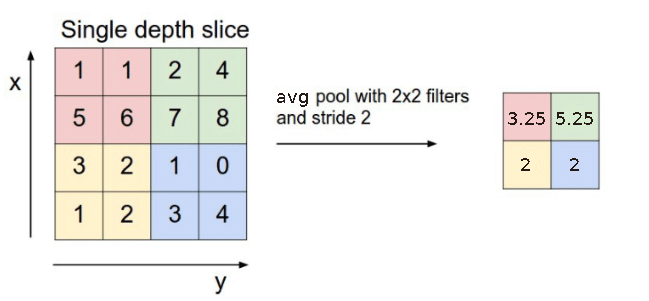
\includegraphics[width=0.9\textwidth]{The-AvgPool-operation.png}
    \caption{\label{fig:avgpool}The average pool operation for a $2 \times 2$ filter with a stride of 2. Figure modified from \protect\citep{MihaiDaniel2020}}
\end{figure}

Due to the large spatial extent of the input predictors, the average pooling layers are defined to have a $4 \times 4$ filter with a stride of 4. Hence, each pooling layer reduces the spatial size of the feature maps by a factor of 4, increasing the domain of influence captured by the receptive field of each pixel in the final feature map of the bottleneck.

\subsubsection{The convolutional block (find new title, same as in methodology)}
The convolutional block from \citet{Ronneberger2015} is adopted for this work, with both the $(3 \times 3)$ filter size and ReLU \citep{Nair2010} activation functions kept. To retain the spatial size of the of the input scene, each convolution is performed with zero-padding, which was omitted in \citet{Ronneberger2015} as it has the potential to create visual artefacts in the border region. Each convolutional block contain two convolutional layers with $2^{6 + n}$ number of output feature maps, where $n$ is the stage of the encoder starting from $n = 0$. The objective of the convolutional block is to detect features and construct feature maps from the incoming tensors, with each filter in the convolutional layers being sensitive only to a single pattern \citep{Fukushima1980}.

The current implementation of the convolutional block deviates from the original U-Net architecture as a normalization layer is added after the each activation function to speed up and stabilize training \citep{Ioffe2015}. Although Batch Normalization has been commonly implemented in deep networks, works such as \citet{Wu2018} demonstrate that the technique exerts drawbacks for small batch size training. In \citet{Wu2018}, the drawbacks in batch normalization are attributed to the normalization statistics computed along the batch dimension of a feature map. Furthermore, \citet{Wu2018} presents an analogous technique for computing normalization statistics, albeit computed along the channel dimension which is divided into connected groups \citep{Wu2018}. The number of groups is set with a hyperparameter $G$. Figure (\ref{fig:BNGN}) visualize the different normalization techniques in \citet{Ioffe2015} and \citet{Wu2018}.

\begin{figure}
    \centering
    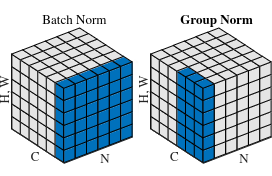
\includegraphics[width=0.35\textwidth]{BNandGN.png}
    \caption{\label{fig:BNGN}Schematic showing a feature map tensor of spatial shape (H,W) with N batches and C channels. The blue pixels are normalized by the same mean and variance. The group normalization hyperparameter $G = 2$. Figure modified from \protect\citep{Wu2018}}
\end{figure}

As increasing the batch size quickly saturates the available memory due to the high resolution predictors, group normalization is adapted for normalizing the feature maps. This follows the results in \citet{Wu2018} where group normalization was shown to reduce network error for small ($<8$) batch sizes. Following the recommendations by \citet{Wu2018}, the hyperparameter $G=32$. 

\subsubsection{Decoder}
The decoder restores the feature maps outputted by the encoder to image-resolution through the use of transposed convolutions \citep{Zeiler2010}. There are a similar amount of transposed convolutional layers as there are pooling layers, yet the number of convolutional blocks is reduced by one when compared to the encoder (see figure (\ref{fig:unet-overview})). The convolutional blocks in the decoder have the same structure as those used in the encoder. Each transposed convolution has a filter size and stride equal to the pooling factor, which has been set to 4. Moreover, the output space for each transposed convolution is $2^{5 - m + n_{\text{max}}}$ starting with $m = 0$ for the first transposed convolutional layer.

\subsubsection{Output layers}
\label{sec:architecture-output}
The feature maps at the final stage of the encoder is fed to the output component of the network. The output component is comprised of $C$ individual output layers as found in \citet{Ronneberger2015} (convolutional layer with $(1 \times 1)$ filter size). However, the number of output channels of each output layer has been reduced to $1$, following the definition of cumulative target contours described in section (\ref{sec:data_targets}). Hence, each output layer facilitates a binary classification task in which each pixel is predicted to belong in the cumulative contour associated with the layer. Finally, each prediction is activated pixel-wise with the sigmoid function (equation (\ref{eq:sigmoid})) which outputs a probability score $\left[0, 1\right]$ for belonging to the predicted contour. The output from the network is on the shape $(C, 1792, 1792, 1)$.
% Dataloader
% Furthermore, as two different model output architectures has been explored, the preprocessing of the targets 

Initially, a more conventional architecture with a single output layer and multiple output categories \citep{Ronneberger2015} was attempted. Conversely, the model applies the softmax activation function (equation (\ref{eq:psoftmax})) to the outputs, which ensures that a single class is selected as most likely. However, due to unsatisfying results during the initial stages of development, further pursue of the architecture was dropped in favour of the above described model. An example prediction visualizing the problematic aspects of the model can be seen in section (\ref{sec:singleoutputmodel}). 

\todo{Nevne noe om hvordan faktiske predictions blir laget}

\subsubsection{Training environment}
\label{sec:train_env}
The model is trained on a GPU workstation with an Nvidia A100 80-Gb GPU available. The largest achievable batch-size in the environment was four. To both speed up training and reduce the memory footprint of the predictors, mixed precision training was utilized \citep{Micikevicius2017}. Mixed precision refers to storing the predictors as half-precision floats, whereas parameters in the model are stored as single-precision floats. Similarly to \citet{Ronneberger2015}, the model weights are HE-initialized \citep{He2015} since the ReLU activation function \citep{Nair2010} is used in the convolutional blocks.

The loss function implemented is the pixelwise Binary Cross Entropy loss, which is an unweighted variation of the loss implemented in \citep{Ronneberger2015} (equation (\ref{eq:unet-loss})) for binary classification tasks. 

\begin{equation}
    \label{eq:loss}
    L = -\frac{1}{N}\sum_{n = 1}^N\sum_{p \in \mathbb{Z}^2}\left(y_p^n\log{(\hat{y}_p^n)} + \left(1 - y_p^n\right)\log{(1 - \hat{y}_p^n)}\right)
\end{equation}

where $N$ is the batch size, $y$ is the true label and $\hat{y}$ is the predicted probability by the model. Subscript $p$ refers to the pixels in $y$ and $\hat{y}$. As a consequence of the architecture described in section (\ref{sec:architecture-output}), the computed losses at each output layer exerts individual contributions to the convolutional layers after the split at the end of the decoder. Furthermore, at the end of the decoder, each loss contribution is reduced to a sum before further propagated through the network during backpropagation.

Motivated by the bias-variance tradeoff described at the end of section (\ref{sec:training-loop}), a validation dataset is used to determine at which epoch the model achieves highest generalizability during training. Further motivated by the regularization effects offered by early stopping \citep{Graves2013}, while still allowing the network to converge further, a model checkpoint technique is deployed where the state of the model weights is stored every time the validational loss achieves a new minimum. As noted, the validation loss is monitored, which will be explored further in coming sections.


\subsection{Hyperparameter tuning and model selection}
Throughout this section, the ice edge displacement metric is referred to frequently. If not otherwise stated, what is referred to is the IIEE of the $(> 10\%)$ contour normalized with respect to the climatological sea ice edge (section \ref{sec:osisafcdr}). Notations such as NIIEE refer to the just described metric. 

\subsubsection{Single output, multiple label model}
\label{sec:singleoutputmodel}
During early stages of model development, an iteration of the deep learning architecture with a single output layer and multiple target labels was developed. Figure (\ref{fig:singleoutmodel}) is an example prediction made with the described model. The categories very open drift ice $(<40\%)$ and open drift ice $(<70\%)$ are not resolved by the model, and persists for all samples (not shown). 

\begin{figure}
    \centering
    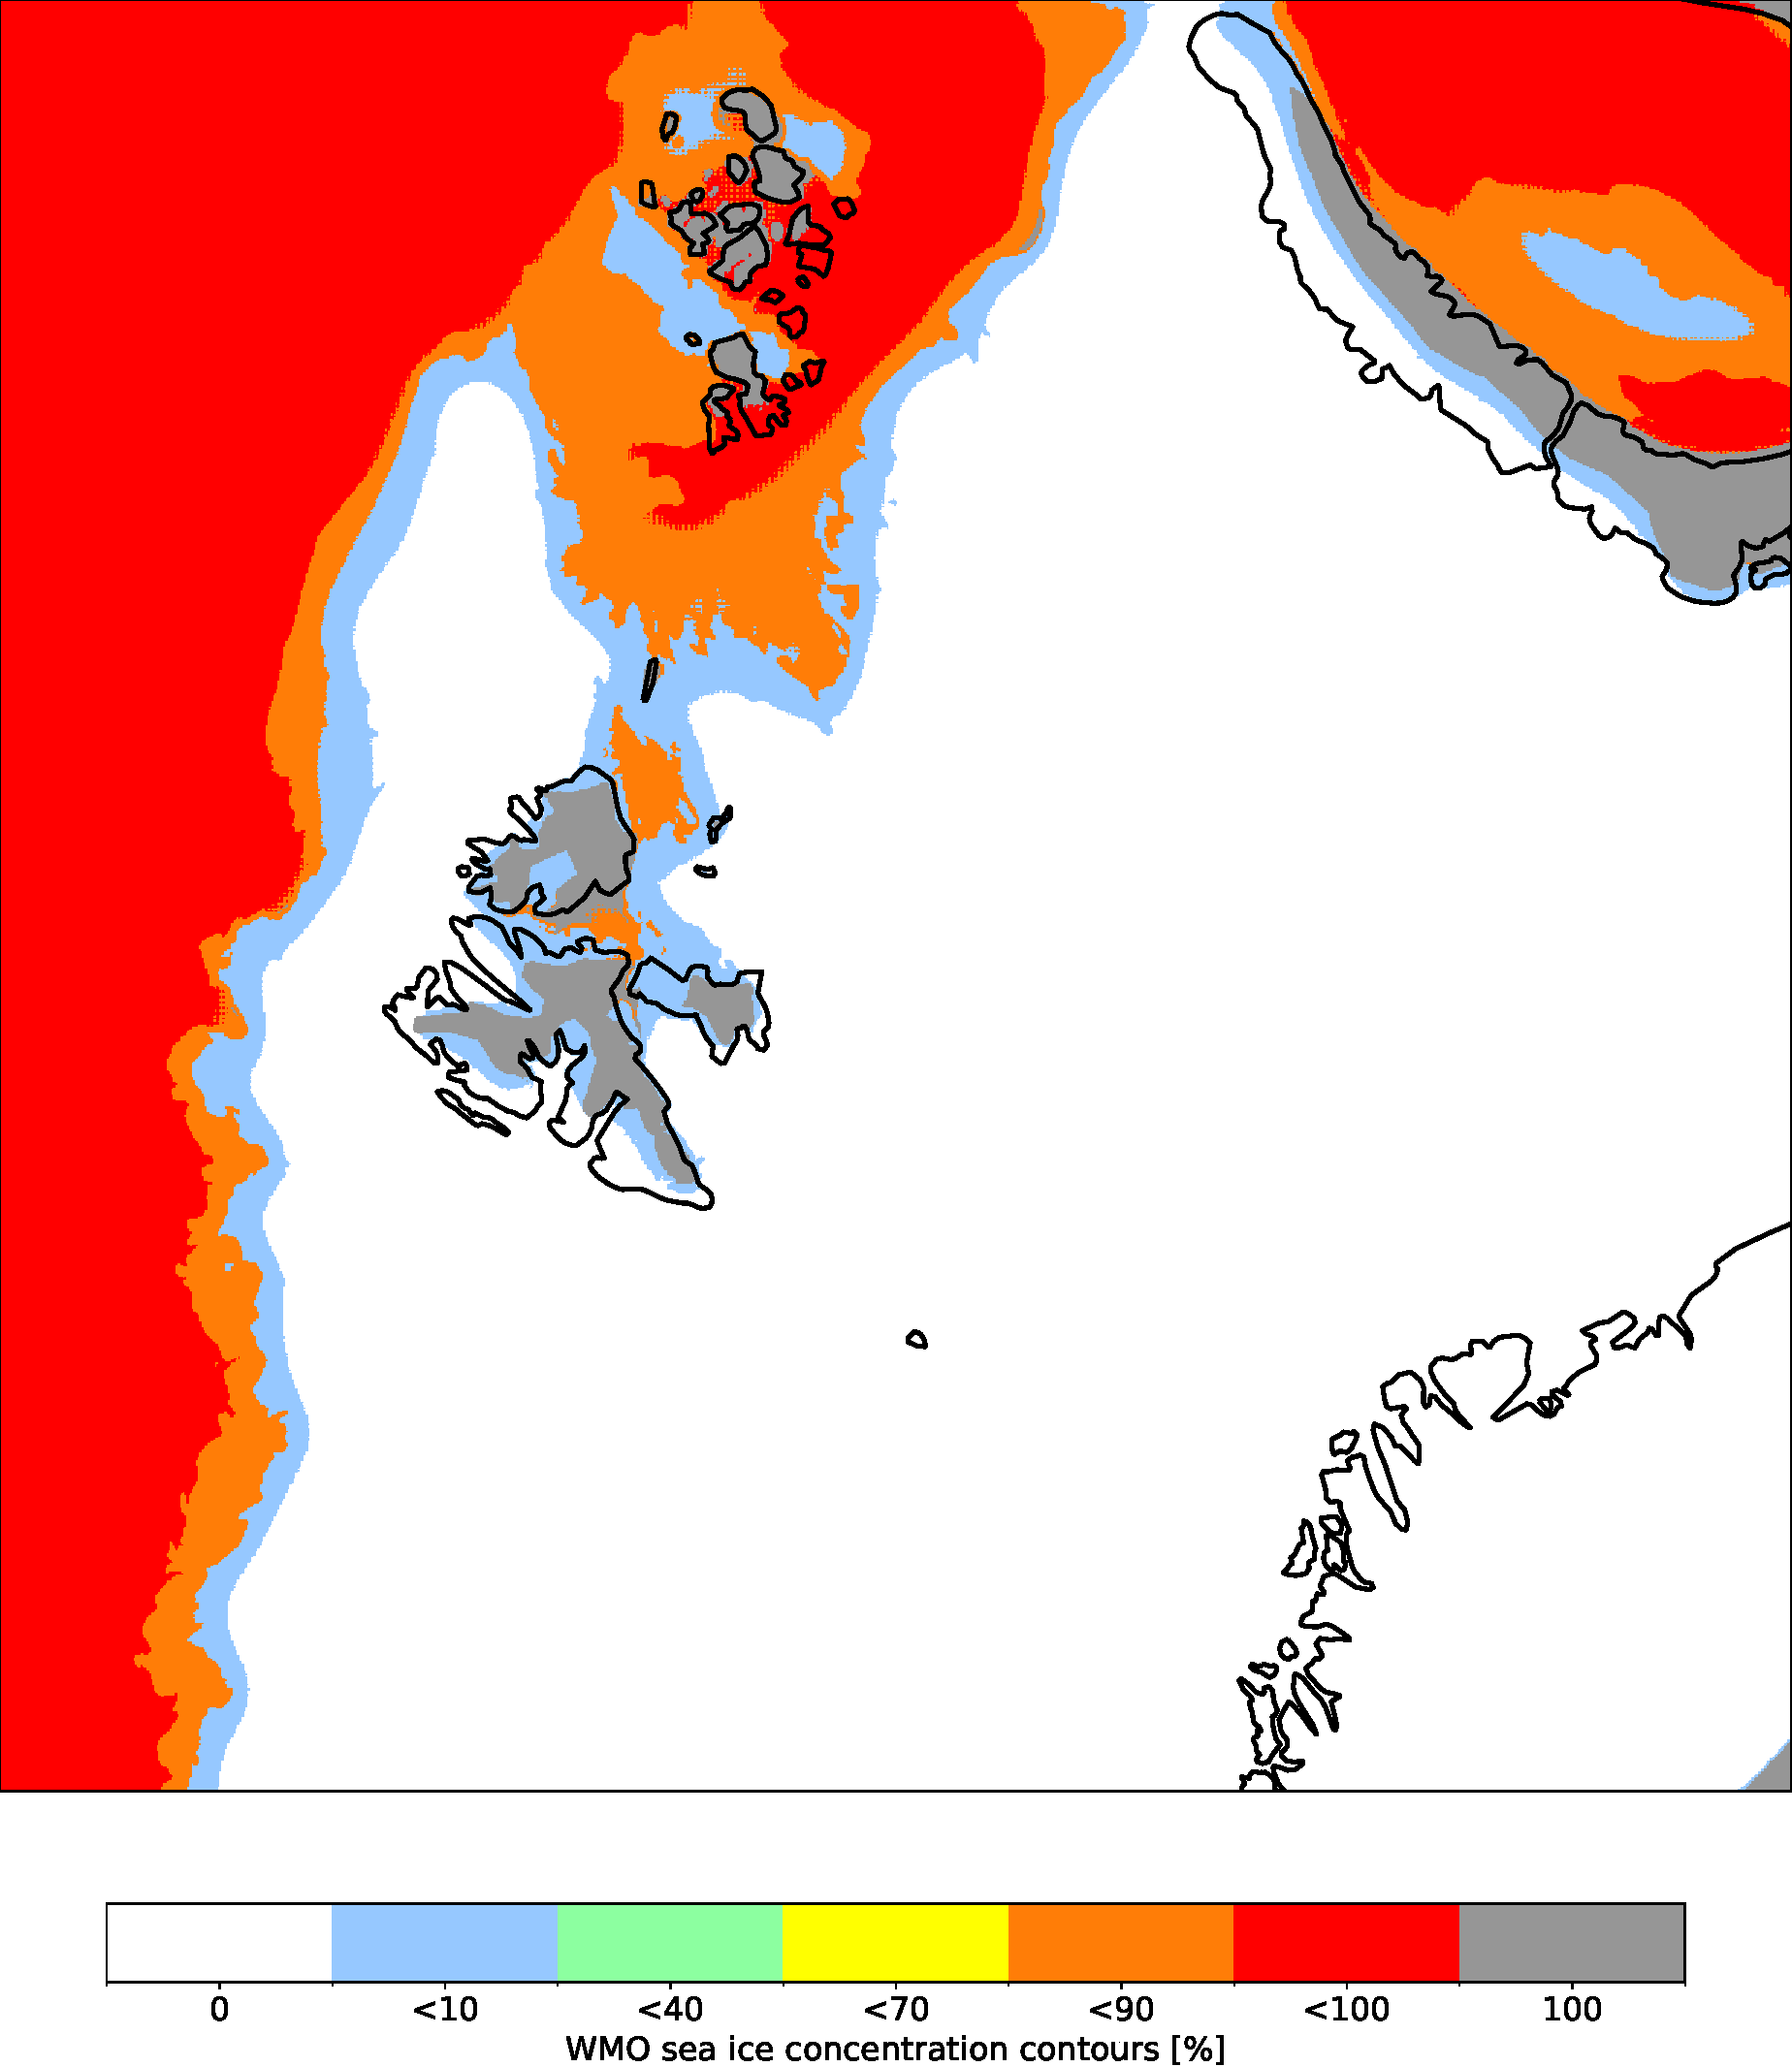
\includegraphics[width=.6\textwidth]{20210106}
    \caption{\label{fig:singleoutmodel}Prediction with a two day lead time, single output multiple labels U-Net 06 Jan 2021.}
\end{figure}

\subsubsection{General training performance}
Training the deep learning system takes $\sim 3\text{h}30\text{min}$ on the GPU workstation, although the training time have varied positively and negatively following driver updates and other non-transparent backend operations. Iterating through the training data takes $\sim 6$ minutes, and the validation data $\sim 8$ minutes for a single epoch. Memory usage varies between $\sim19.4$ and $\sim55$ gb, and scales with the depth of the unet. With a pre-trained model, performing a single prediction on a workstation CPU (AMD EPYC 7282 16-Core) takes $\sim 6$ seconds, while on a laptop CPU (Intel(R) Core(TM) i7-8565U 8-Core) takes $\sim 30$ seconds.

To determine the optimal learning rate and U-Net depth, a grid search was conducted across variations of the aforementioned variables. The result is shown in figure \ref{fig:gs}. It can be seen from the figure that the validation loss increases with U-Net depth. At the same time, the validation loss also increases when the learning rate deviates from $0.001$.

\begin{figure}
    \centering
    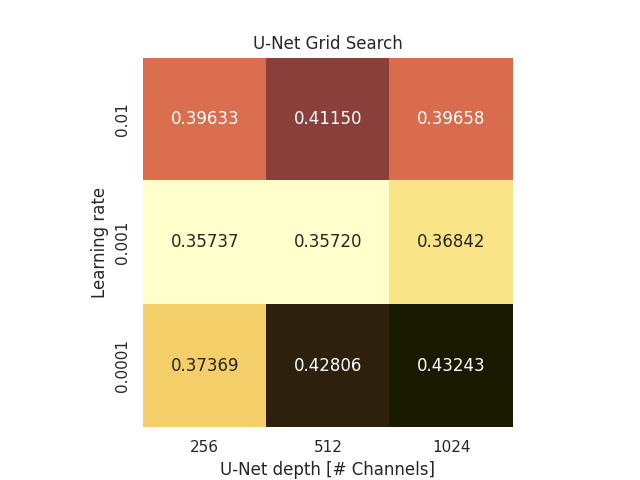
\includegraphics[width=.8\textwidth]{grid_search}
    \caption{\label{fig:gs}Grid search performed over variations of the learning rate as well as an increasing U-Net depth (represented by the number of feature maps at the at the final convolutional block). Each cell contain the minimum obtained validation loss of its respective combination which is associated with the best validation performance during training.}
\end{figure}

Training curves for the model in figure \ref{fig:gs} which achieved a loss of 0.35737 ($\text{lr} = 0.001$, $\text{U-Net depth} = 256$) are shown in figure \ref{fig:loss_curve_from_gs}. The figure plots both the training and validation loss, as well as a third curve which keeps track of the current minimum validation loss. The lowest validational loss is achieved at epoch 17. 

\begin{figure}
    \centering
    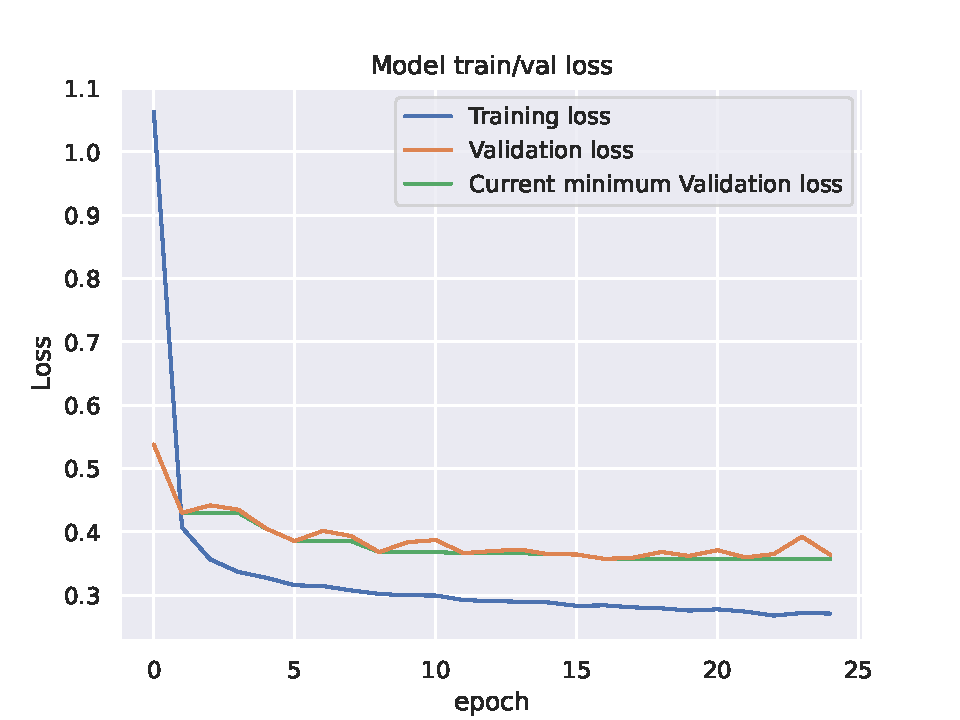
\includegraphics[width=\textwidth]{loss_curve_best_model_gs}
    \caption{\label{fig:loss_curve_from_gs}Training and validation loss from the model attaining lowest validation loss in Figure (\ref{fig:gs}). The current minimum validation loss is also displayed.}
\end{figure}

Figure \ref{fig:256_1024_compare} is intended as a demonstration of the impact model depth have on the predictions. Both models are trained on the same data, and the best model for both training procedures is selected according to section \ref{sec:train_env}. Both models resolve the scene comparatively, with mean annual statistics of ice edge displacement error being 28.2 km for the model in figure \ref{fig:gs_middle_left} and 30.7 km for the model in figure \ref{fig:gs_middle_right}. The total number of trainable parameters in the 256 architecture is $\sim 2.4$ million, where $\sim 1.15$ million is located in the encoder and $\sim 1.25$ million in the decoder. The rightmost model in figure \ref{fig:256_1024_compare}, which have a depth of 1024 filters, contain $\sim 16$ times as many parameters as the model with a depth of 256 filters, with a total of $\sim39 $ million parameters. Decomposing the total number of parameters into encoder and decoder results in $\sim 19$ million parameters in the encoder and $\sim 20$ million parameters in the decoder. The receptive field of the bottleneck (final feature map in the encoder) for both models is calculated using equation \ref{eq:receptivefield}. The model with a depth of 256 has an encoder with a theoretical receptive field of 145 pixels in each spatial dimension, whereas the model with a depth of 1024 has an encoder with a theoretical receptive field of 2385 pixels in each direction. For the second model, a receptive field of 2385 results in the entire input scene being used as context for each pixel in the final encoder feature map. Note that the theoretical receptive field is invariant to the input shape.

\begin{figure}
    \centering
    \begin{subfigure}{0.49\textwidth}
        \centering
        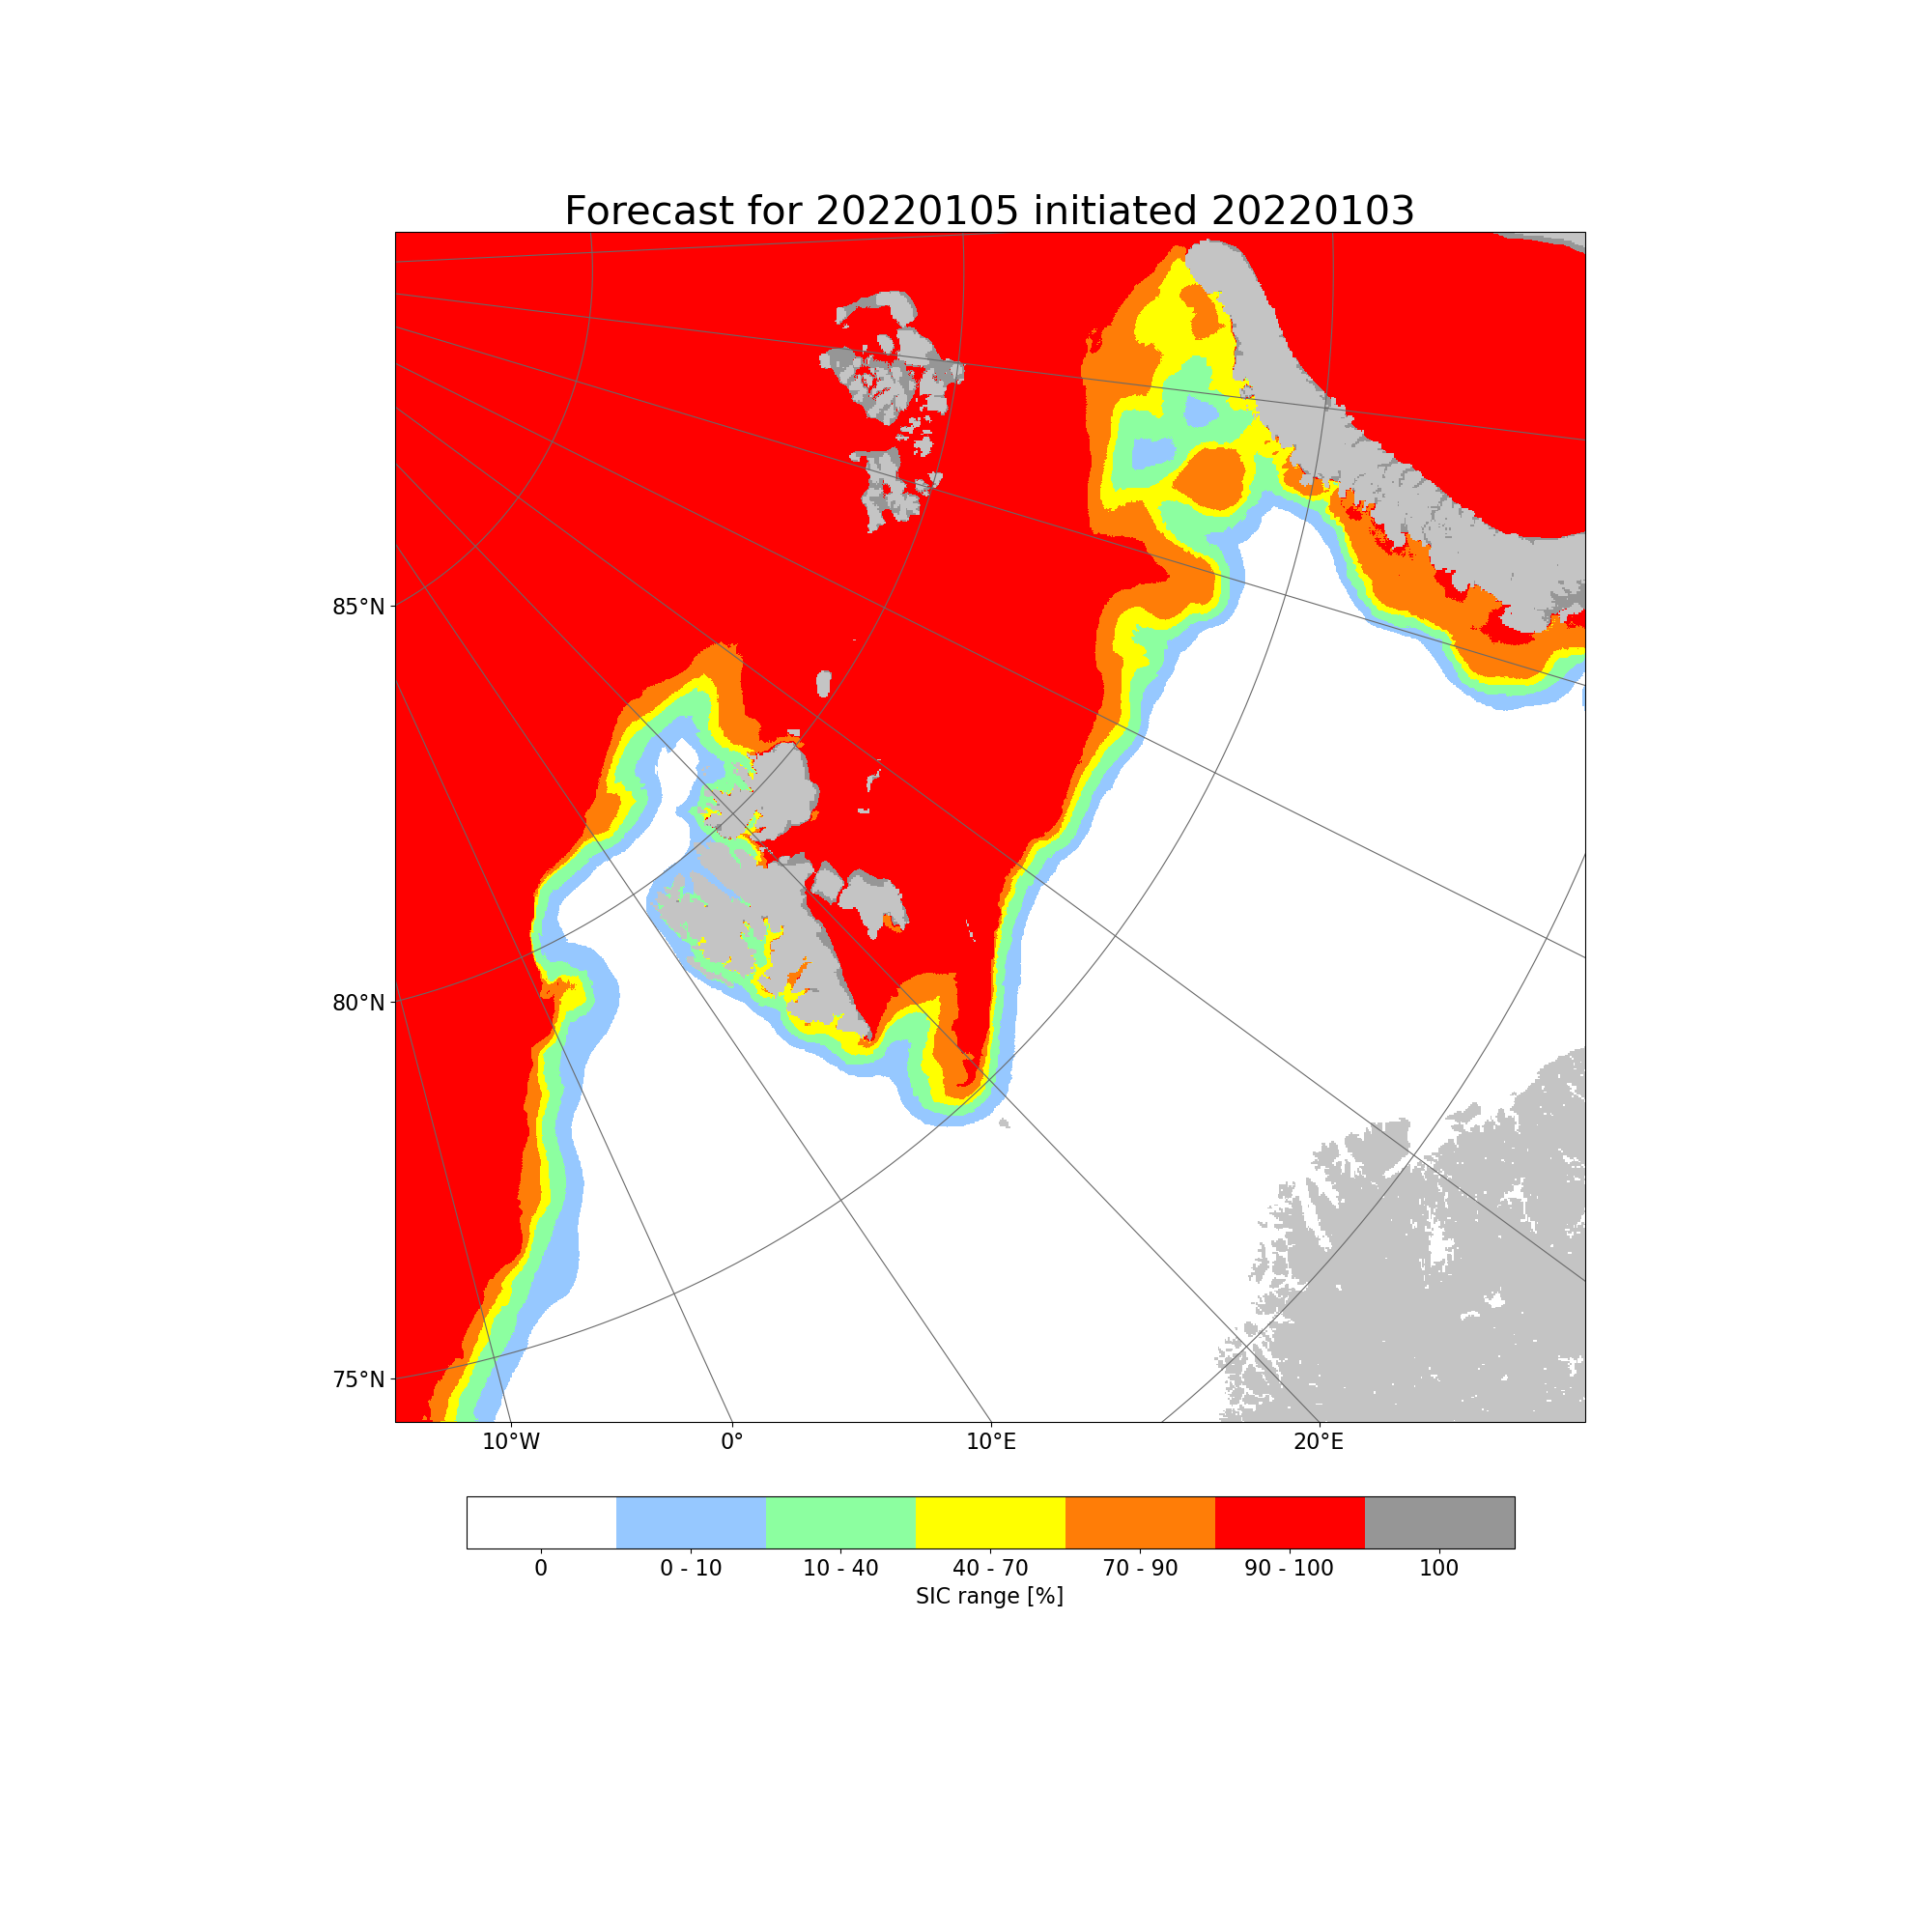
\includegraphics[width=\textwidth, trim=85mm 85mm 85mm 50mm, clip]{unet_256_jan}
        \caption{Prediction with a 2 day lead time for 05 Jan 2022 using a deep learning model with lr = 0.001 and depth 256.}
        \label{fig:gs_middle_left}
    \end{subfigure}\hfill
    \begin{subfigure}{0.49\textwidth}
        \centering
        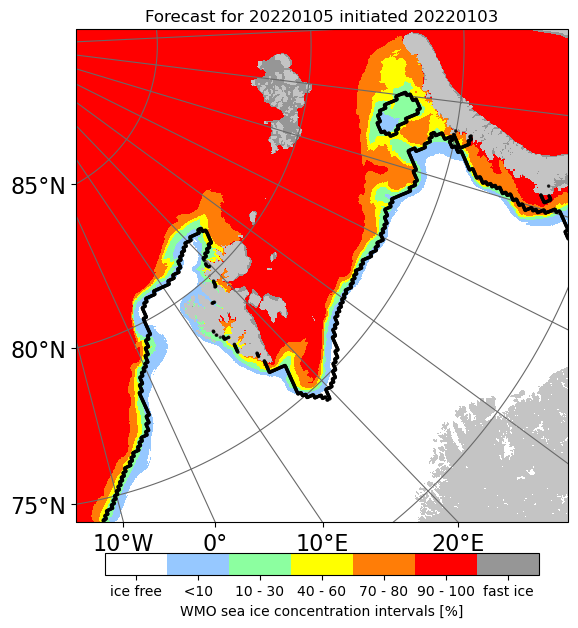
\includegraphics[width=\textwidth, trim=85mm 85mm 85mm 50mm, clip]{unet_1024_jan}
        \caption{Prediction with a 2 day lead time for 05 Jan 2022 using a deep learning model with lr = 0.001 and depth 1024.}
        \label{fig:gs_middle_right}
    \end{subfigure}
    \caption{Prediction of the same date with two different models with parameters as in figure \ref{fig:gs}. The model in figure (a) contains $\sim 2.4$ million parameters, and achieves a mean annual ice edge displacement ($>10\%$ contour) of 28.2 km. The model in figure (b) contains $\sim 39$ million parameters, and achieves a mean annual ice edge displacement of 30.7 km}
    \label{fig:256_1024_compare}
\end{figure}

A full year of forecasts, where each month is represented by the first prediction made that month using a 2 day lead time model and 256 architecture is shown in figure \ref{fig:timeseries}. Figure \ref{fig:timeseries} also visualizes the sea ice edge computed from OSI SAF ssmis observations at 10km spatial resolution. The figure is intended as an example of the predictive capabilities of the model across the entire test dataset. 

\begin{figure}
    \centering
    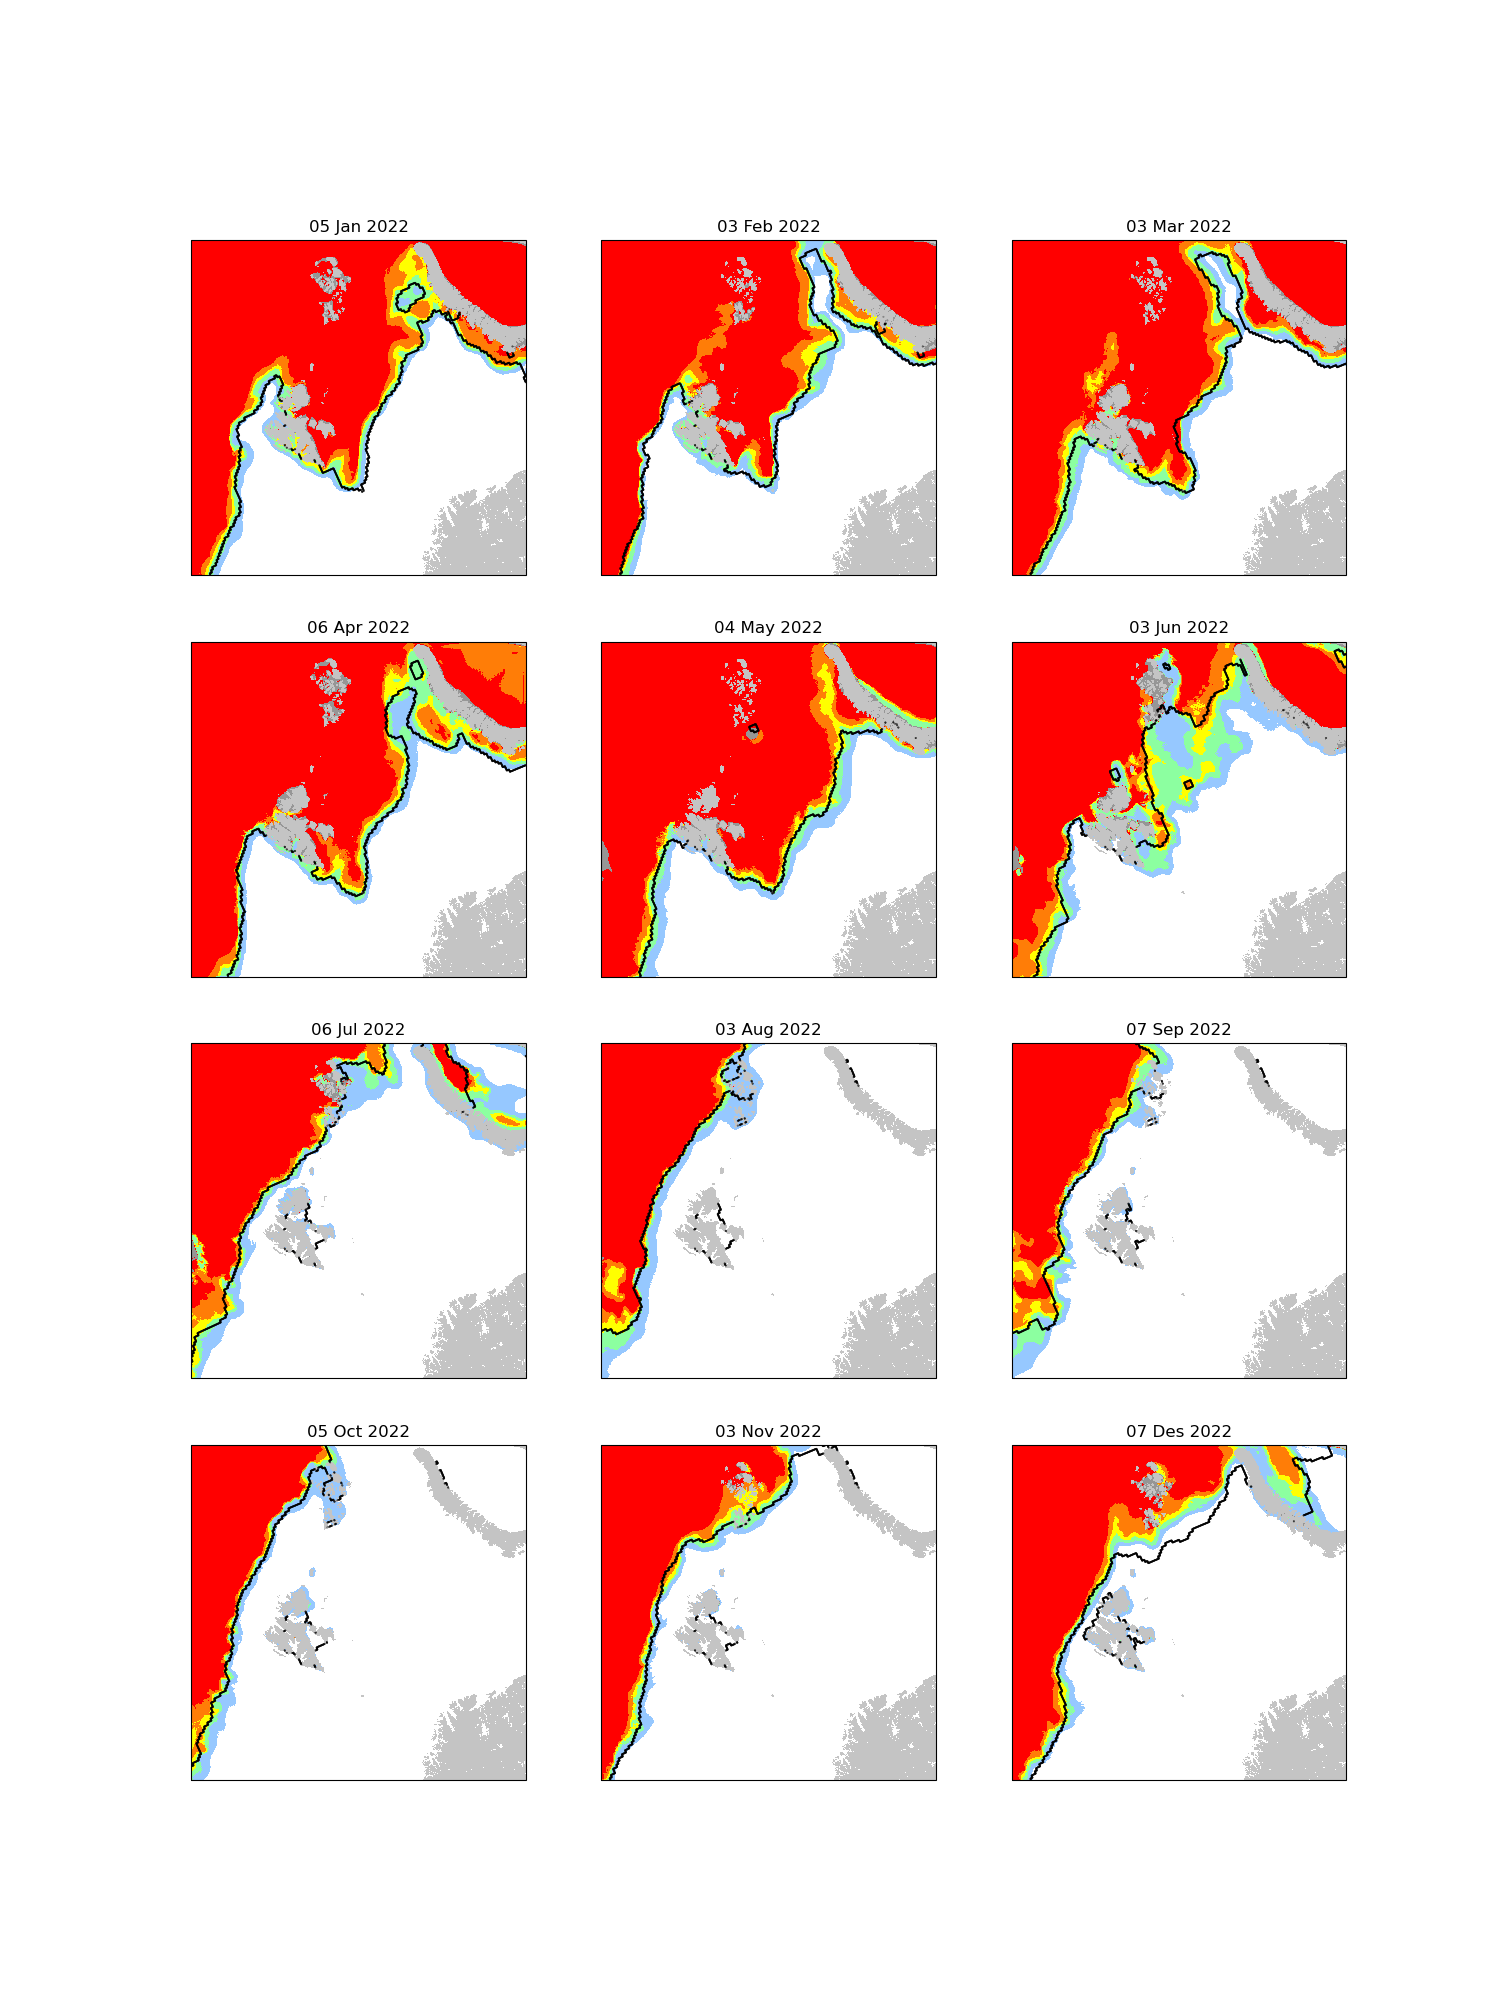
\includegraphics[width=.86\textwidth]{Forecast_time_series}
    \caption{\label{fig:timeseries}Prediction with a 2 day lead time given the first available ice chart each month of 2022. The black line is the 15\% ice edge computed from OSI SAF ssmis. The figure exemplifies the predicitve capabilities of the model. Subplots for each month exemplifies seasonal variability of the model. The WMO color code is preserved, no colorbar is shown.}
\end{figure}

The effect of training across varying lead time is shown in figure \ref{fig:lead_times}. From figure \ref{fig:lead_times} a), it can be seen that both persistence and the deep learning forecast increase their mean annual NIIEE with increasing lead times. It can also be seen that persistence achieve a higher mean annual NIIEE than the deep learning model for all lead times. Figure \ref{fig:lead_times} b) show that the forecast improvement increase with the lead time, which follows the divergence between the deep learning and persistence NIIEE curves in a) which show a diverging pattern. 

\begin{figure}
    \centering
    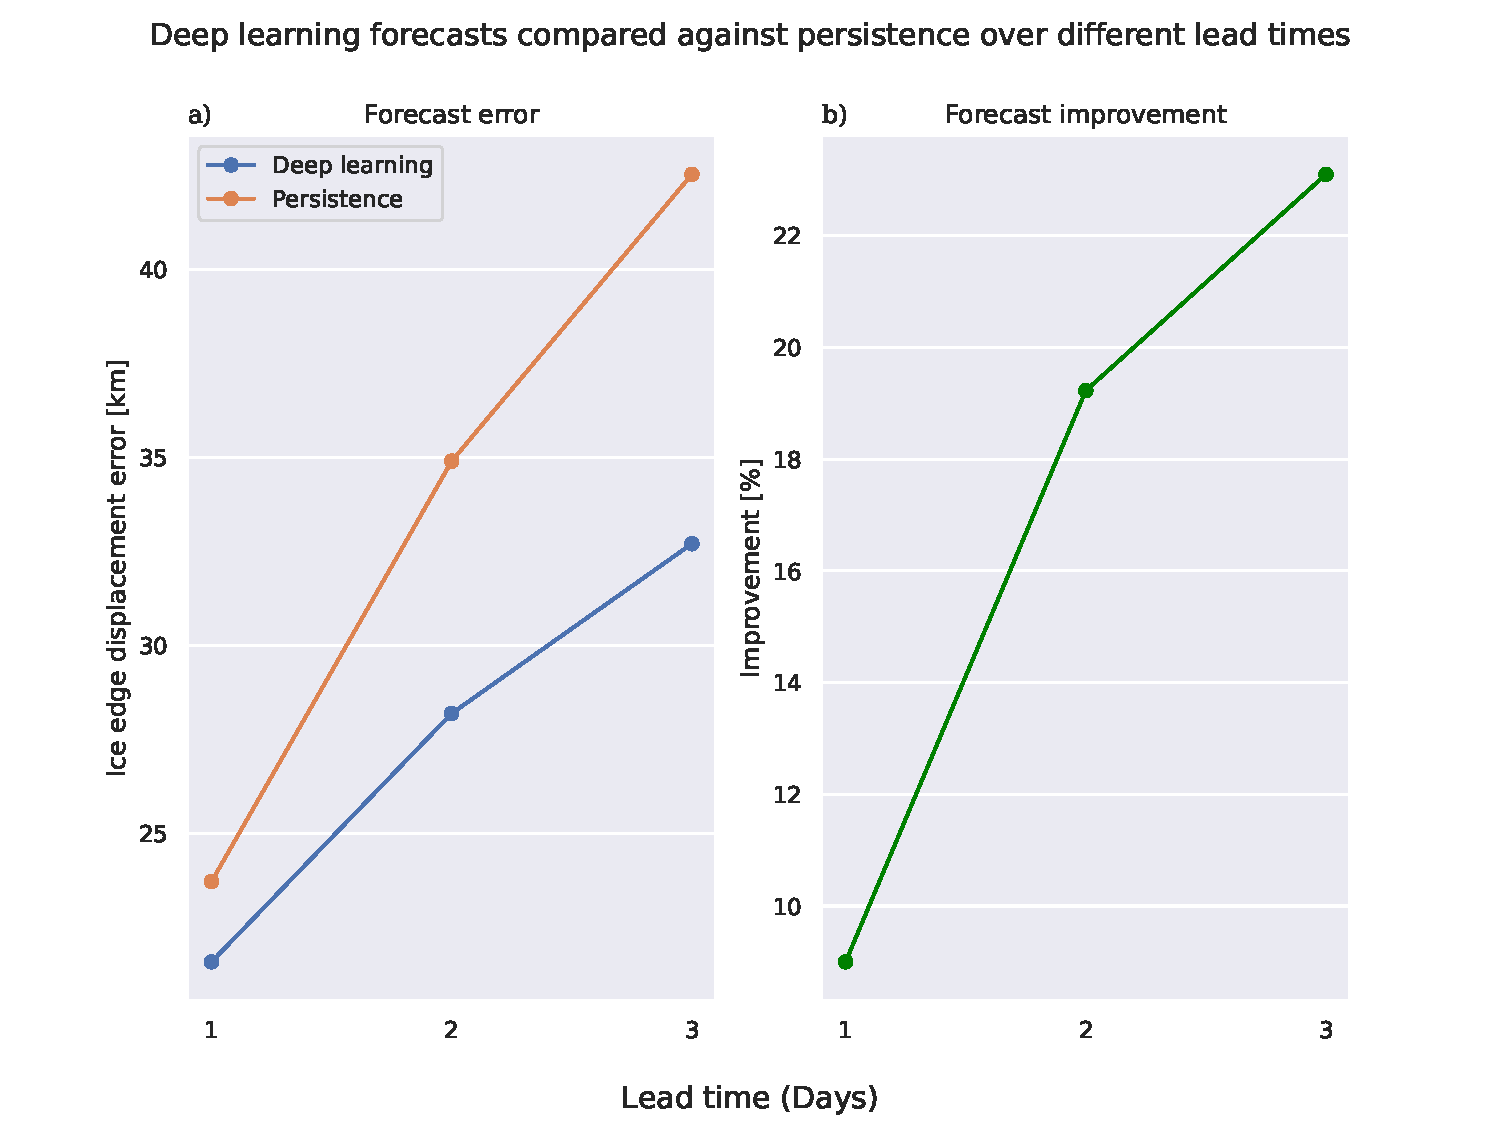
\includegraphics[width=\textwidth]{lead_times.pdf}
    \caption{\label{fig:lead_times}Comparing the effect of training the deep learning system against varying target lead time. The ice edge displacement reported in subfigure a) is the normalized IIEE with regards to the $(> 10\%)$ contour. The improvement in subfigure b) is computed in favour of the deep learning forecast.}
\end{figure}

An inspection on the effect of appending additional years to the core (2019 and 2020) training data is summarized in figure \ref{fig:append_years}. Both validation loss and NIIEE is shown in figure \ref{fig:append_years}. The model trained with a training dataset starting in 2016 and including all years up until including 2020 has higher validation loss (2021) and NIIEE (2022) than the other models in figure \ref{fig:append_years}. The model trained with 2017 up until including 2020 achieves the lowest score on both monitored metrics.

\begin{figure}
    \centering
    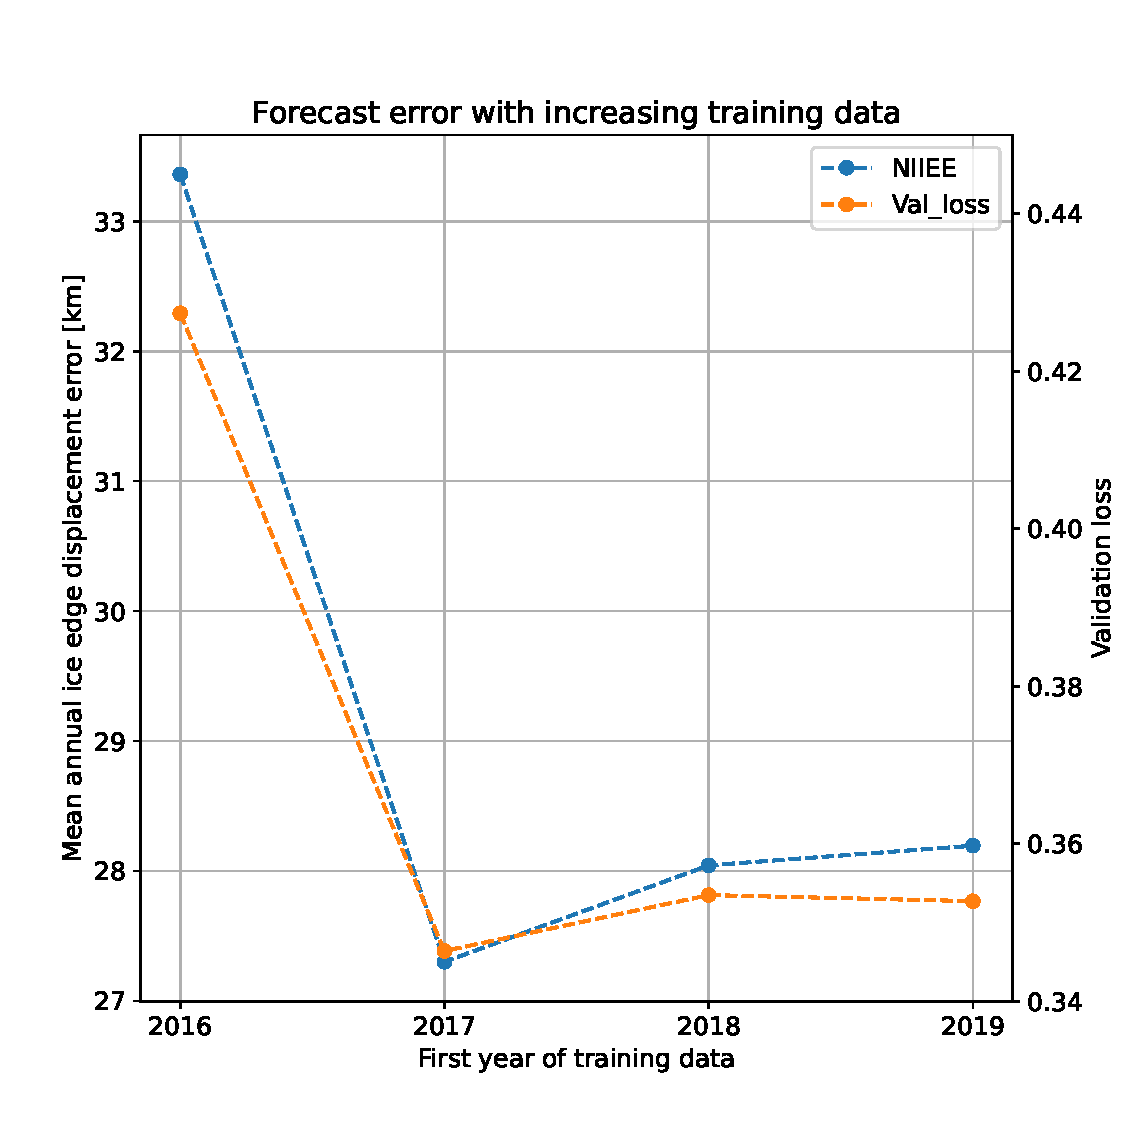
\includegraphics[width=.9\textwidth]{years_start.pdf}
    \caption{\label{fig:append_years}The lines visualize the relationship between start year for the training data (upper bound is always 2020) with the ice edge displacement error for the $(> 10\%)$ contour and validation loss.}
\end{figure}

The effect of the non-linear activation function was assessed by training a model were the activation functions were replaced with a linear mapping. The mean annual NIIEE on the test set was 41.35 km, which is 13.15km more than the benchmark model with a mean annual NIIEE of 28.20 km. A qualitative prediction made with the model can be seen in figure \ref{fig:linear_model}. 

\begin{figure}
    \centering
    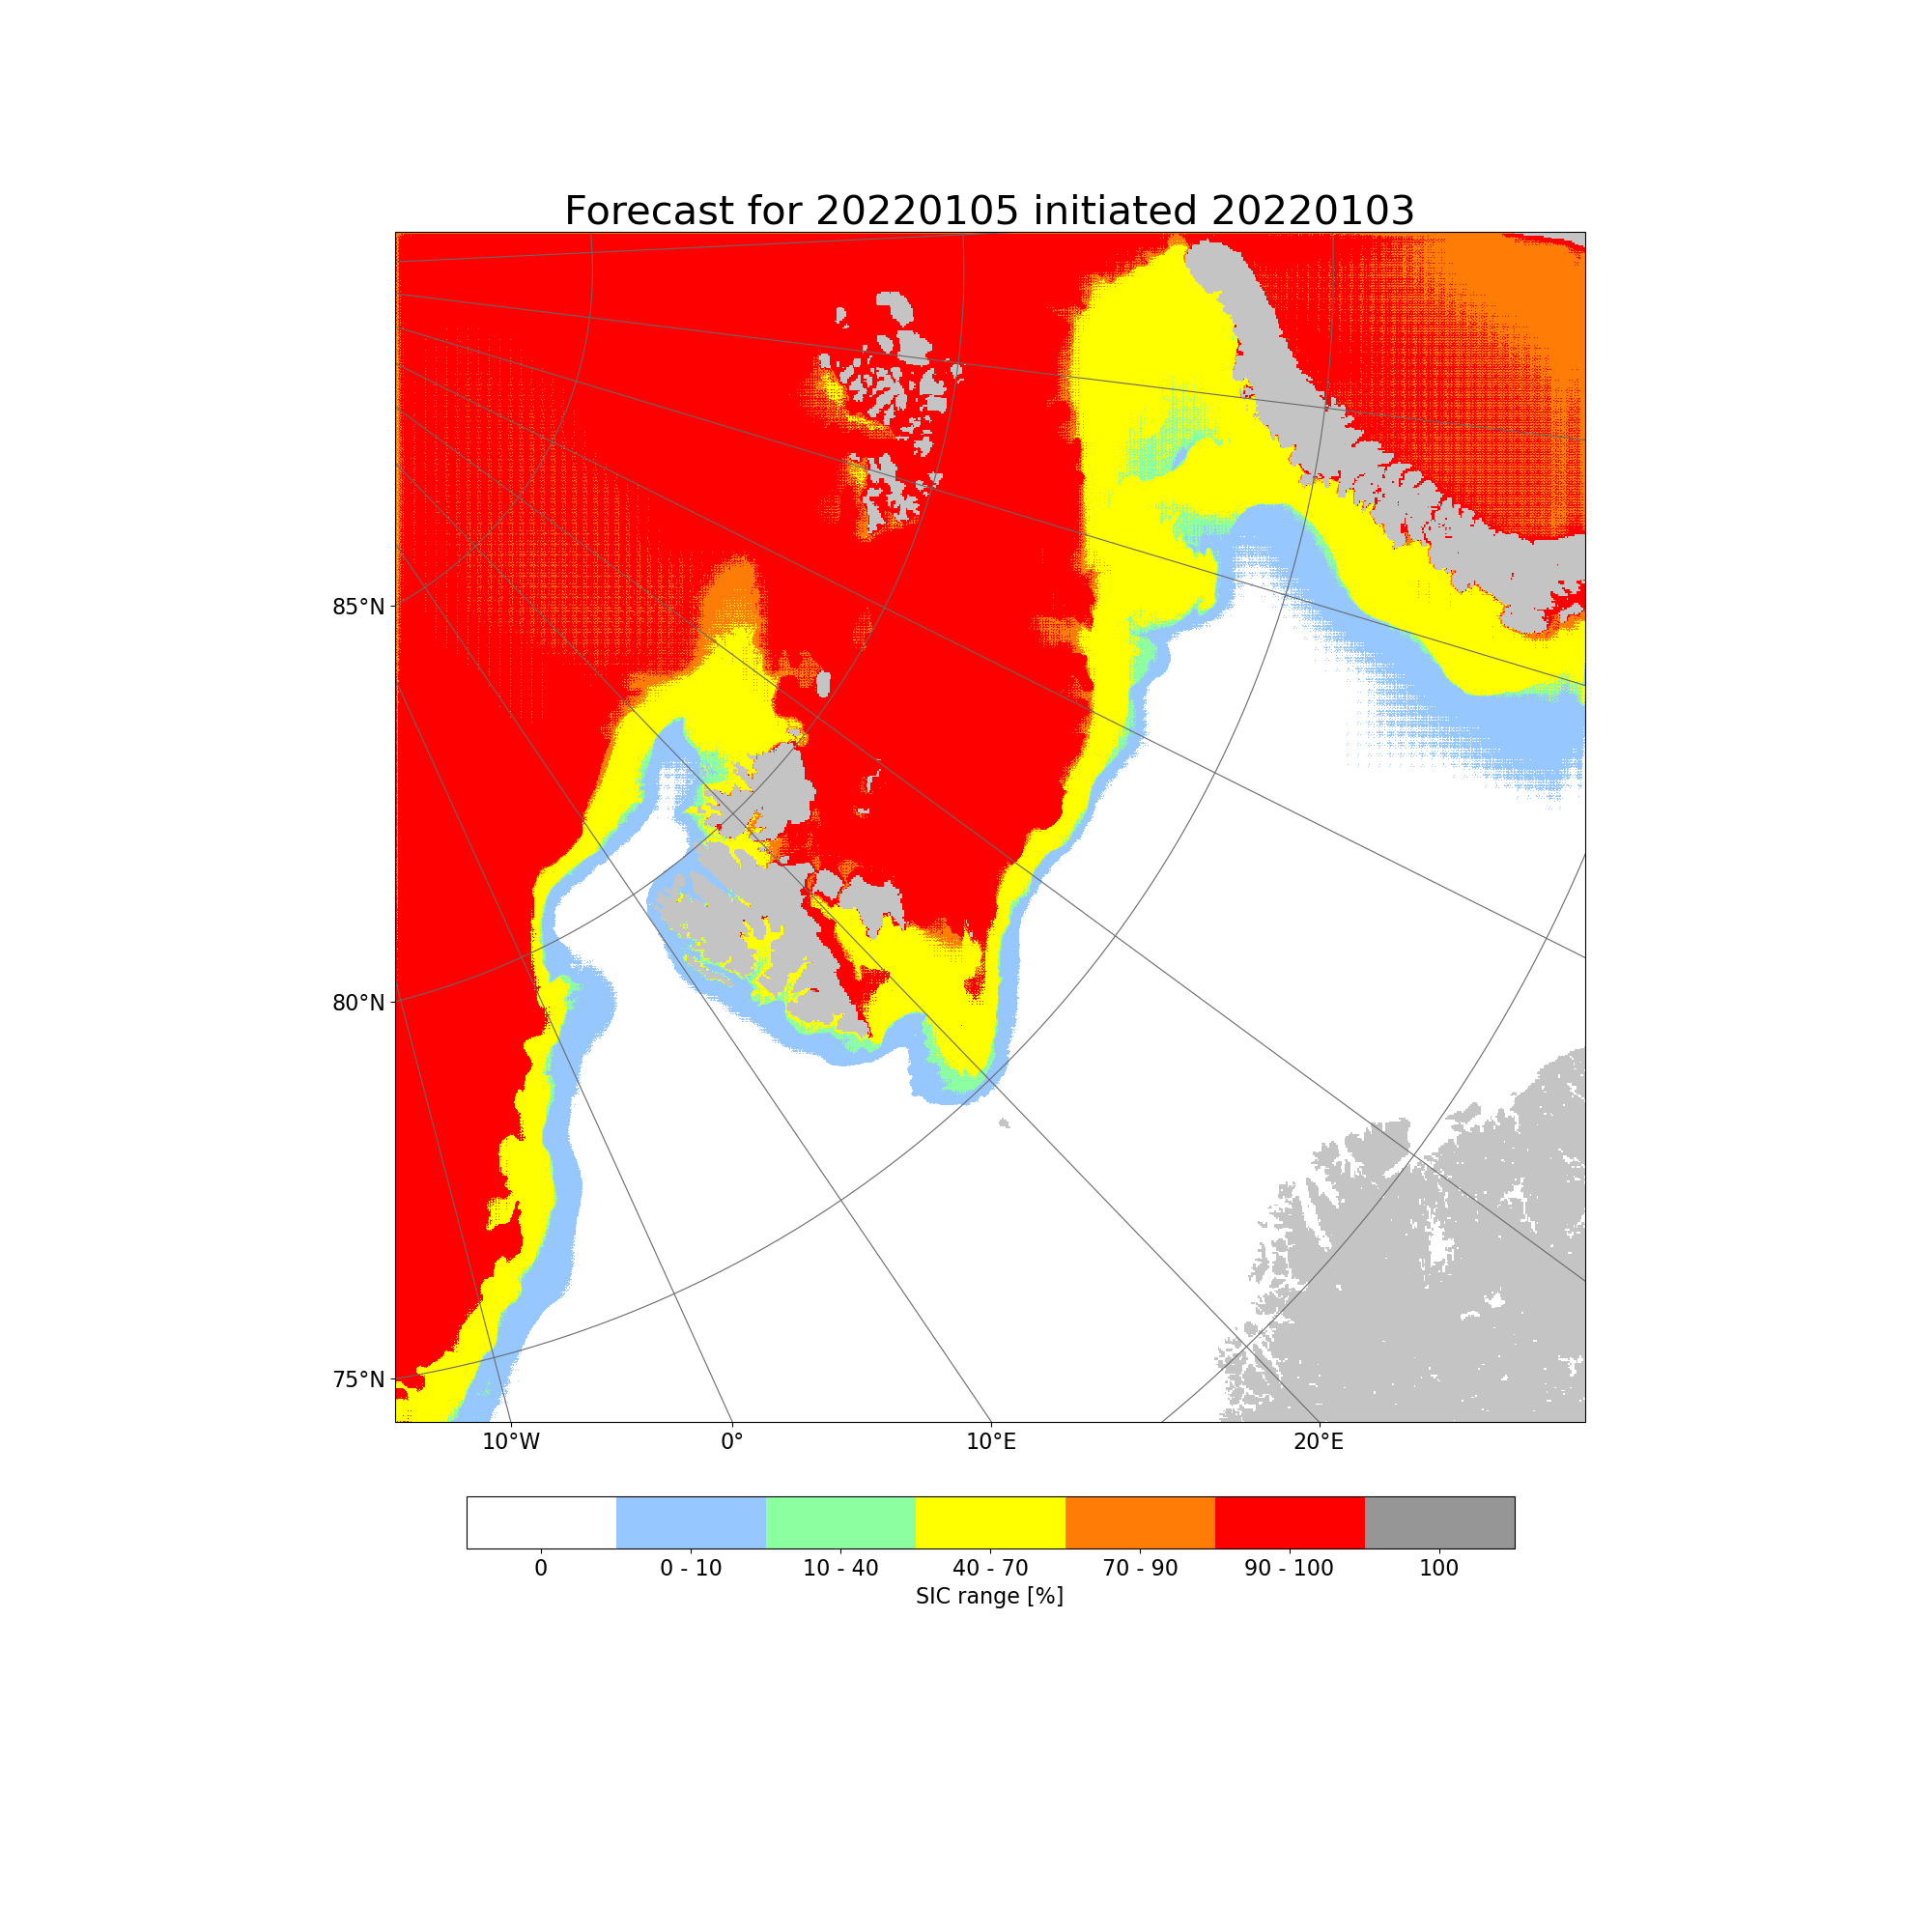
\includegraphics[width=\textwidth, trim=85mm 85mm 85mm 50mm, clip]{linear_model_jan}
    \caption{\label{fig:linear_model}Prediction with a two day lead time model, where all non-linear activation functions were replaced with linear mappings. The figure aim to qualitatively demonstrate a prediction made with a linear model. FIX CATEGORY LABELS}
\end{figure}

\subsubsection{Modifying predictor related hyperparameters}
The effect of setting all pixels in the predictor ice chart covered by the land mask as ice free open water (category 0) and reducing the number of ice chart classes was inspected. When replacing all land covered predictor pixels to ice free open water, a mean annual NIIEE of 29.72 km was achieved. 

When reducing the number of possible classes in the ice chart, two contours were modified. The $(< 10\%)$ sea ice concentration contour was set to ice free open water, whereas the $(100\%, \text{land fast ice})$ contour was set to the class below $(< 100\%, \text{very close drift ice})$. The model was still trained similarly to other models, and achieved a mean annual NIIEE of 28.61 km.  

\subsubsection{Connecting validation loss with IIEE}
Section \ref{sec:train_env} described how model selection is performed, where the model that performs best on the validation dataset (2021) with regards to minimizing the loss is selected. This subsection presents a result where the IIEE displacement error \citep{Goessling2016, Melsom2019} with respect to the $(>10\%)$ contour is performed. 

The IIEE was Normalized with respect to a climatological Ice Edge length derived from ten years of OsiSaf data as described in section \ref{sec:osisafcdr}. When iterating through the validational dataset after an epoch is completed, all validational predictions are used to compute the IIEE with respect to their associated ground truth label. The results are summarized in figure \ref{fig:val_loss_iiee}

\begin{figure}
    \centering
    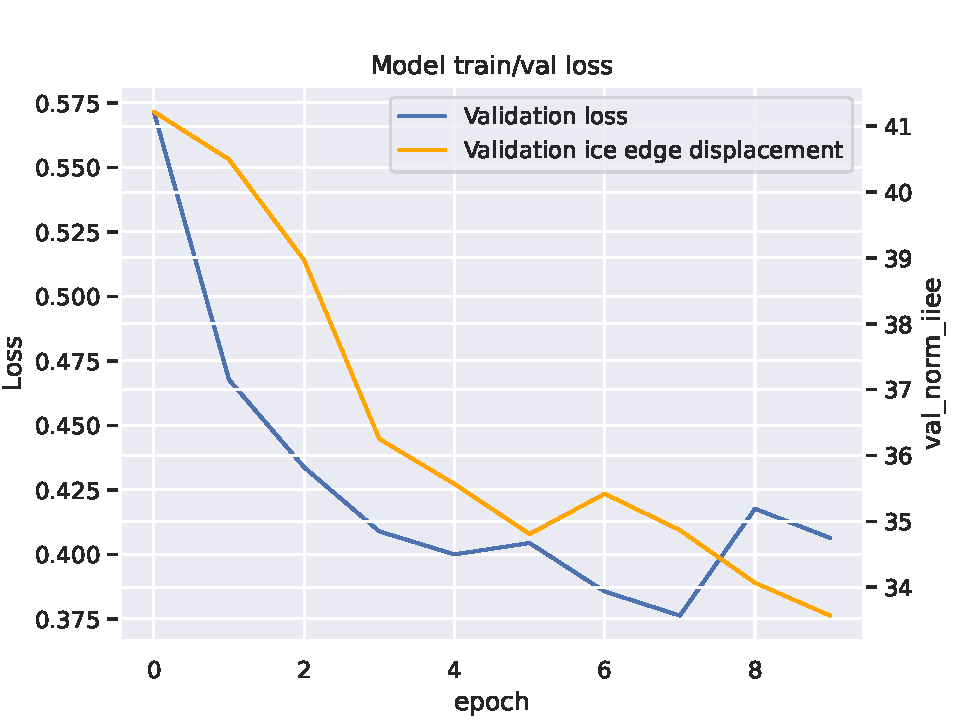
\includegraphics[width=\textwidth]{val_loss_iiee}
    \caption{\label{fig:val_loss_iiee}Validation loss and validation normalized ice edge displacement as a function of epoch. A training environment with a 2 day lead time was used.}
\end{figure}

The correlation between the validation loss and validation normalized ice edge displacement reported in figure \ref{fig:val_loss_iiee} is 0.82. Moreover, training the model for 10 epochs with the previously described IIEE validation scheme took 21 hours. A single IIEE validation iteration took 2 hours. 

\biblio
\end{document}